\documentclass[11pt]{article}

\usepackage{booktabs}
\usepackage{dcolumn} 
\usepackage{epstopdf}
\usepackage{fourier}
\usepackage{fullpage}
\usepackage{graphicx}
\usepackage{hyperref}
\usepackage{longtable} 
\usepackage{natbib}
\usepackage{rotating}
\usepackage{tabularx}
\usepackage{amsmath}
\usepackage{algorithmic} 
\usepackage{algorithm2e}

\hypersetup{
  colorlinks = TRUE,
  citecolor=blue,
  linkcolor=red,
  urlcolor=black
}

\newcommand{\important}[1]{\textcolor{blue}{\textbf{ #1}}}
\newcommand{\quantclaim}[1]{\textcolor{red}{\textbf{ #1}}}
\newcommand{\starlanguage}{Some TK scale about statistical significance.}

\begin{document} 

\title{Getting a Shift or Getting the Shaft ?: \\
  The Labor Market Consequences Algorithmic Scheduling}

\date{\today}

\author{John J. Horton \\
  Leonard N. Stern School of Business\\
  New York University \footnote{Author contact information, datasets and code are currently or will be available at \href{http://www.john-joseph-horton.com/}{http://www.john-joseph-horton.com/}. } }
\maketitle

\begin{abstract}
  \noindent
  Many retail firms now use algorithmic, demand-aware approaches for staffing.
  Critics argue that this approach shifts risks and costs to workers and reduces total hours worked;
  several states and cities are considering (or have passed ordinances) to guarantee workers more predictable work schedules.
  Despite these concerns, I find no evidence that the work patterns of retail workers has changed substantially in the last 10 years, during which algorithmic scheduling has become commonplace. 
  As a possible reconciliation for the lack of any reduction in hours-worked, I show that it is theoretically ambiguous whether hours-worked would rise of fall in response to greater employer precision in forecasting demand---it depends on whether the firm was over- or under-staffing in response to uncertain demand. 
    %\noindent JEL J01, J24
\end{abstract} 

\section{Introduction}

Many kinds of firms must staff their locations in response to time varying demand:
retail locations, restaurants, service businesses, customer service centers and so on. 
Both over-staffing and under-staffing are costly to the firm and so presumably firms try to predict their demand and then staff accordingly.
While a competent manager could probably do reasonably well simply by observation---a coffee shop will soon learn that mornings and busy and afternoons slow---but other factors that are, in principle, predictable, might more difficult for any individual manager to learn.
As a result, many firms now use machine learning techniques to learn about time-varying demand, incorporating a number of factors unavailable to any individual manager, and then staffing on the basis of those predictions. 

While increased predictability is presumably is good for the firm, the effects on workers is less obvious and in fact, algorithmic scheduling has come under fire.
Some argue that these systems shift the risk inherent in variable demand away from firms and towards workers.
Given that workers are presumably less able to bear risk that firms---particularly those working in relatively low-paying retail establishments paying hourly wages---even if efficient, the utility loss could be great.
This possibility has attracted popular press attention and has lead to some policy changes. 
\footnote{
\href{http://www.nytimes.com/interactive/2014/08/13/us/starbucks-workers-scheduling-hours.html}{
  New York Times, ``Working Anything but 9 to 5'':``Scheduling Technology Leaves Workers with Hours of Chaos''}
Boston Globe,
\href{https://www.bostonglobe.com/2015/07/20/sen-warren-worker-schedules-should-more-predictable/lVt0dtlVaEGCsqT7SXztRJ/story.html}{ ``Worker schedules should be more predictable, Warren says''}
}

In the competetive labor market model, workers would have to be compensated for taking on this extra hours risk.
However, if firms have some bargaining power, then they might be better able to pass through these costs to workers. 

In this paper, I consider a simple model in which the firm has to choose a staffing level in response to stochastic demand.
When wages are relatively higher, firms tend to over-staff, whereas when wages are low, they tend to under-staff.
When prediction gets better, demand for labor can either increase of decrease, depending on whether the firm was under- or over-staffing earlier. 

\subsection{Literature}

Flexible Schedules: What are we Trading Off to Get Them? 
http://www.bls.gov/mlr/2001/03/art3full.pdf


Did Adam Smith mention variance in chapter on what determines wages?
\cite{smith1999wealth}

\cite{trejo1991effects}
\cite{crepon2002employed}
\cite{hamermesh2000demand}
\cite{skuterud2007identifying}

% http://www.jstor.org/stable/2006639?seq=1#page_scan_tab_contents

\section{Empirics}
The criticism of algorithmic scheduling is that it creates schedules that are bad for workers.
Several kinds of bad shifts have been identified.
One is the ``split shift'' where a worker works for several hours, then has a long (unpaid) break followed by another shift.
A similar problem is a combination of shifts that leaves little time for rest, such as being asked to both open and close a store, or a ``clopening.'' 
Finally, some workers have reported being send home if demand is slack, without being paid. 

Many of these kinds of bad shifts would not ``show up'' in an aggregate measures of hours-worked. 
For example, to detect a clopening one would need the start and end times of periods of work.
Fortunately, this kind of data is available in the American Time Use Survey (ATUS).
It contains the the by-minute activities of a large number of CPS respondents.
The link between the CPS and the ATUS allows us to look at the work schedules of those workers with occupations thought to be affected by algorithmic scheduling. 

\subsection{Sample}
The sample consists of all ATUS respondents from 2013 to 2014 reporting that their occupation was ``retail worker'' (Cenus occupation code 4760). 
The respondents in the ATUS were originally participants in the CPS.
They are later asked to describe their previous day in great detail, which I will use to explore their work day.

\subsection{Hours worked} 

Figure~\ref{fig:hours_reporting} shows the fraction of the sample reporting the various Census-hours worked categogies each year.
These numbers are from the CPS data, not from the activity diary / ATUS. 
There is now obvious pattern, with all measures basically flat over time.
Note in particular that the fractions reportin that hours vary (either part-time or full-time) are both flat and make up a small fraction of the workers. 

\begin{figure}[h]
\centering 
\caption{Fraction of retail workers reporting various number of hours per week} \label{fig:hours_reporting}
\begin{minipage}{0.90 \linewidth}
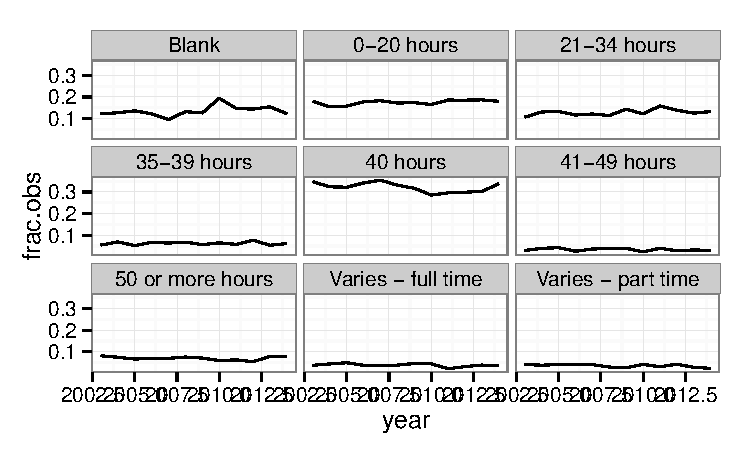
\includegraphics[width = \linewidth]{./plots/hours_reporting.pdf}
\\
\emph{Notes}: The sample consists of all ATUS respondents each year reporting working in a retail occupation.
The y-axis in each panel is the fraction of respondents reporting that answer that year to the question about how many hours they worked per week.
The x-axis is the year of the survey. 
\end{minipage} 
\end{figure}

% 
% Table created by stargazer v.5.2 by Marek Hlavac, Harvard University. E-mail: hlavac at fas.harvard.edu
% Date and time: Mon, Oct 19, 2015 - 09:21:44 AM
\begin{table}[!htbp] \centering 
  \caption{Respondent reported hours category} 
  \label{tab:hired_rate} 
\begin{tabular}{@{\extracolsep{5pt}}lccc} 
\\[-1.8ex]\hline 
\hline \\[-1.8ex] 
 & \multicolumn{3}{c}{\textit{Dependent variable:}} \\ 
\cline{2-4} 
\\[-1.8ex] & Varies - part time & Varies - full time & High hours \\ 
\\[-1.8ex] & (1) & (2) & (3)\\ 
\hline \\[-1.8ex] 
 Year & $-$0.001$^{*}$ & $-$0.001 & $-$0.005$^{**}$ \\ 
  & (0.001) & (0.001) & (0.001) \\ 
  & & & \\ 
 Constant & 2.284$^{*}$ & 1.626 & 9.578$^{***}$ \\ 
  & (1.061) & (1.095) & (2.815) \\ 
  & & & \\ 
\hline \\[-1.8ex] 
Observations & 9,966 & 9,966 & 9,966 \\ 
R$^{2}$ & 0.0005 & 0.0002 & 0.001 \\ 
\hline 
\hline \\[-1.8ex] 
\end{tabular}
\begin{minipage}{0.9\textwidth} 
 \emph{Notes:} Here are some notes.
 \end{minipage}
\end{table}


\subsection{Working on the sample day}
Not all retail workers in the ATUS report working on the work activity reporting day.
TK: Which day of the week is the sample taken on?
Figure~\ref{fig:frac_working} shows the fraction of the ATUS sampe that reports at least one spell of work on their work diary day. 
It peaked at about 90\% in 2007 and then has declined since, with the 2014 at about 75\%.
These measures are fairly imprecise, however. 

\begin{figure}[h]
\centering 
\caption{Fraction of self-identified retail workers working on the ATUS activity diary day} \label{fig:frac_working}
\begin{minipage}{0.95 \linewidth}
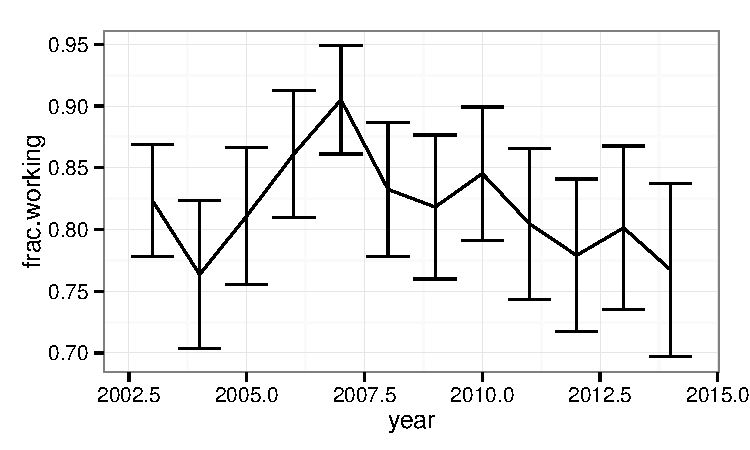
\includegraphics[width = \linewidth]{./plots/frac_working.pdf}
\\
\emph{Notes}: Fraction of ATUS respondents reporting doing at least some paid work on their ATUS survey day.  
\end{minipage} 
\end{figure}

\subsection{Shifts}

Each ATUS respondent records precisely what they were doing at different parts of the day. 
Figure~\ref{fig:shifts_2014} plots the 24 hours covered by the activity diary for the sample, with time when the respondent was working filled in black.
The purpose of this plot is to illustrate the nature of the ATUS activity diary and convey the variation in patterns of work. 

\begin{figure}[h]
\centering 
\caption{Shift visualizations for retail workers in 2014} \label{fig:shifts_2014}
\begin{minipage}{0.75 \linewidth}
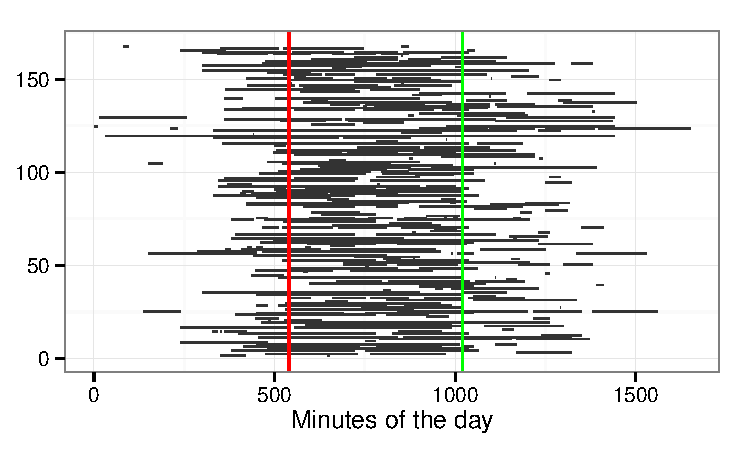
\includegraphics[width = \linewidth]{./plots/scheduling_2014.pdf}
\\
\emph{Notes}: The black blocks represent continuous periods of work.  
\end{minipage} 
\end{figure}

Figure~\ref{fig:mean_minutes_worked} plots the average minuted-worked per day for ATUS retail workers.
There is no detectable pattern in cumulative hours-worked.

\begin{figure}[h]
\centering 
\caption{ATUS-calculated mean minutes worked per day over time, conditional upon working for retail workers}
\label{fig:mean_minutes_worked}
\begin{minipage}{0.75 \linewidth}
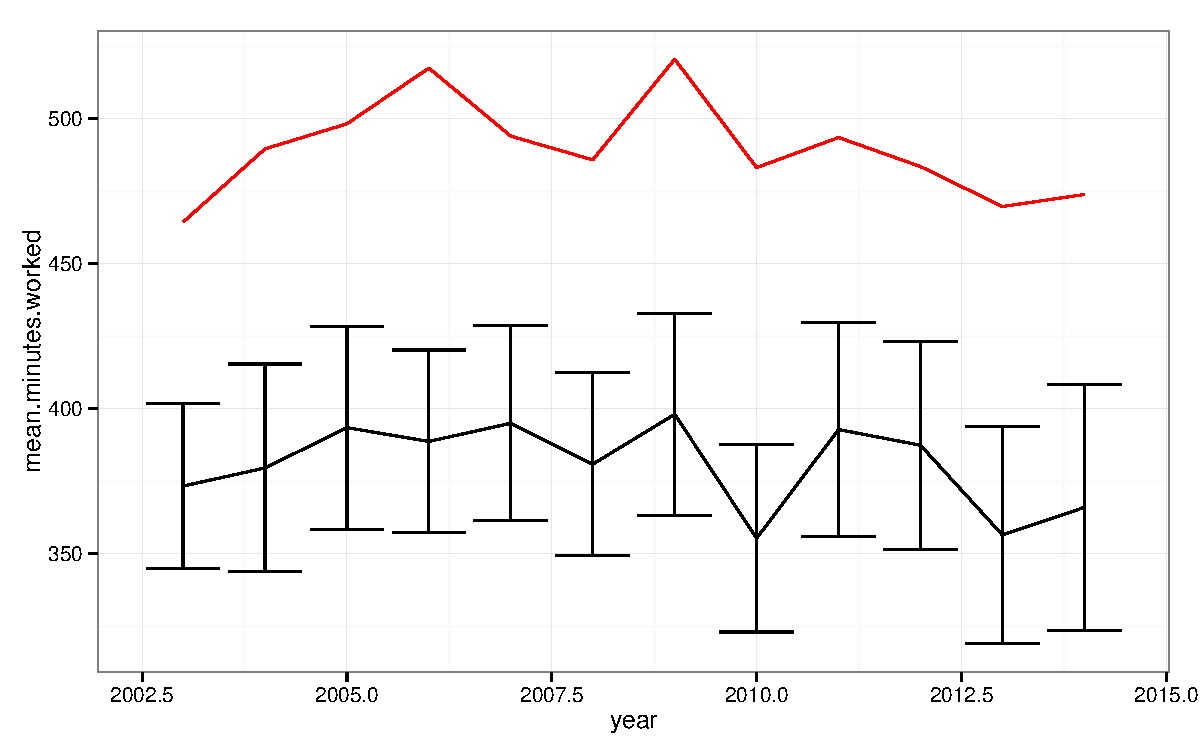
\includegraphics[width = \linewidth]{./plots/mean_minutes_worked.pdf}
\\
\emph{Notes}: Mean minutes worked per day for ATUS retail worker respondents. 
\end{minipage} 
\end{figure}

\subsection{Start and end times}

The ``clopening'' could show up as early start times or later end time.
However, Figure~\ref{fig:clopening} shows no strong pattern in average work day start and end times.

\begin{figure}[h]
\centering 
\caption{Mean day start and day end times for retail workers, by year} \label{fig:clopening}
\begin{minipage}{0.90 \linewidth}
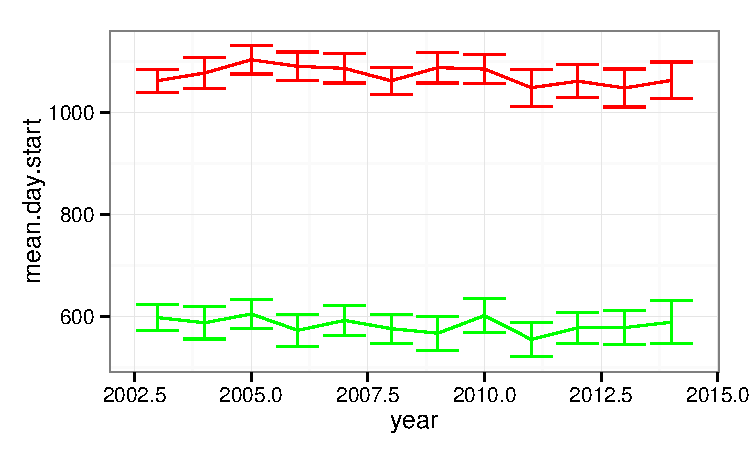
\includegraphics[width = \linewidth]{./plots/clopening.pdf}
\\
\emph{Notes}: 
\end{minipage} 
\end{figure}

\section{Model}
A firm must choose an number of workers to work a shift in response to demand, $d$. 
Each unit of demand, if met by a worker, provides revenue $p$.
Each worker on a shift can serve one unit of demand. 
The firm's profit are 
\begin{align}
 \pi(L) = p \cdot \min \{L, d\} - w L   
\end{align} 
where $w$ is the wage of a worker and $L$ is the number of workers used on the shift. 
For the firm to be willing to hire anyone, $p > w$. 
Demand is random variable, with 
\begin{align}
 d = d_0 + \epsilon   
\end{align}
where $\mathbf{E}[\epsilon] = 0$ and $V(\epsilon) = \sigma$.

We can think of the firm's problem as first choosing $L = d_0$ and then adjusting this headcount by $\Delta L$.  
This adjustment can either be $\Delta L < 0$, meaning the firm chooses to under-staff or $\Delta L > 0$, where the firm chooses to over-staff.
Figure~\ref{fig:choice} illustrates the firm's problem, showing the change in profits for different realizations of $\epsilon$, for a particular choice of $\Delta L$.
As drawn, the firm has chosen to over-staff ($\Delta L > 0)$.
This means that even when $\epsilon = 0$, the firm suffers a loss in profits of $w \Delta L$.
However, for all values of $\epsilon > \Delta L$, the firm gets $(p - w)\Delta L$. 
The sloped line as a slope of $p$. 

\begin{figure}[h]
\centering 
\caption{Firm's revenue for different realized demand shocks, given a staffing decision} \label{fig:choice}
\begin{minipage}{0.75 \linewidth}
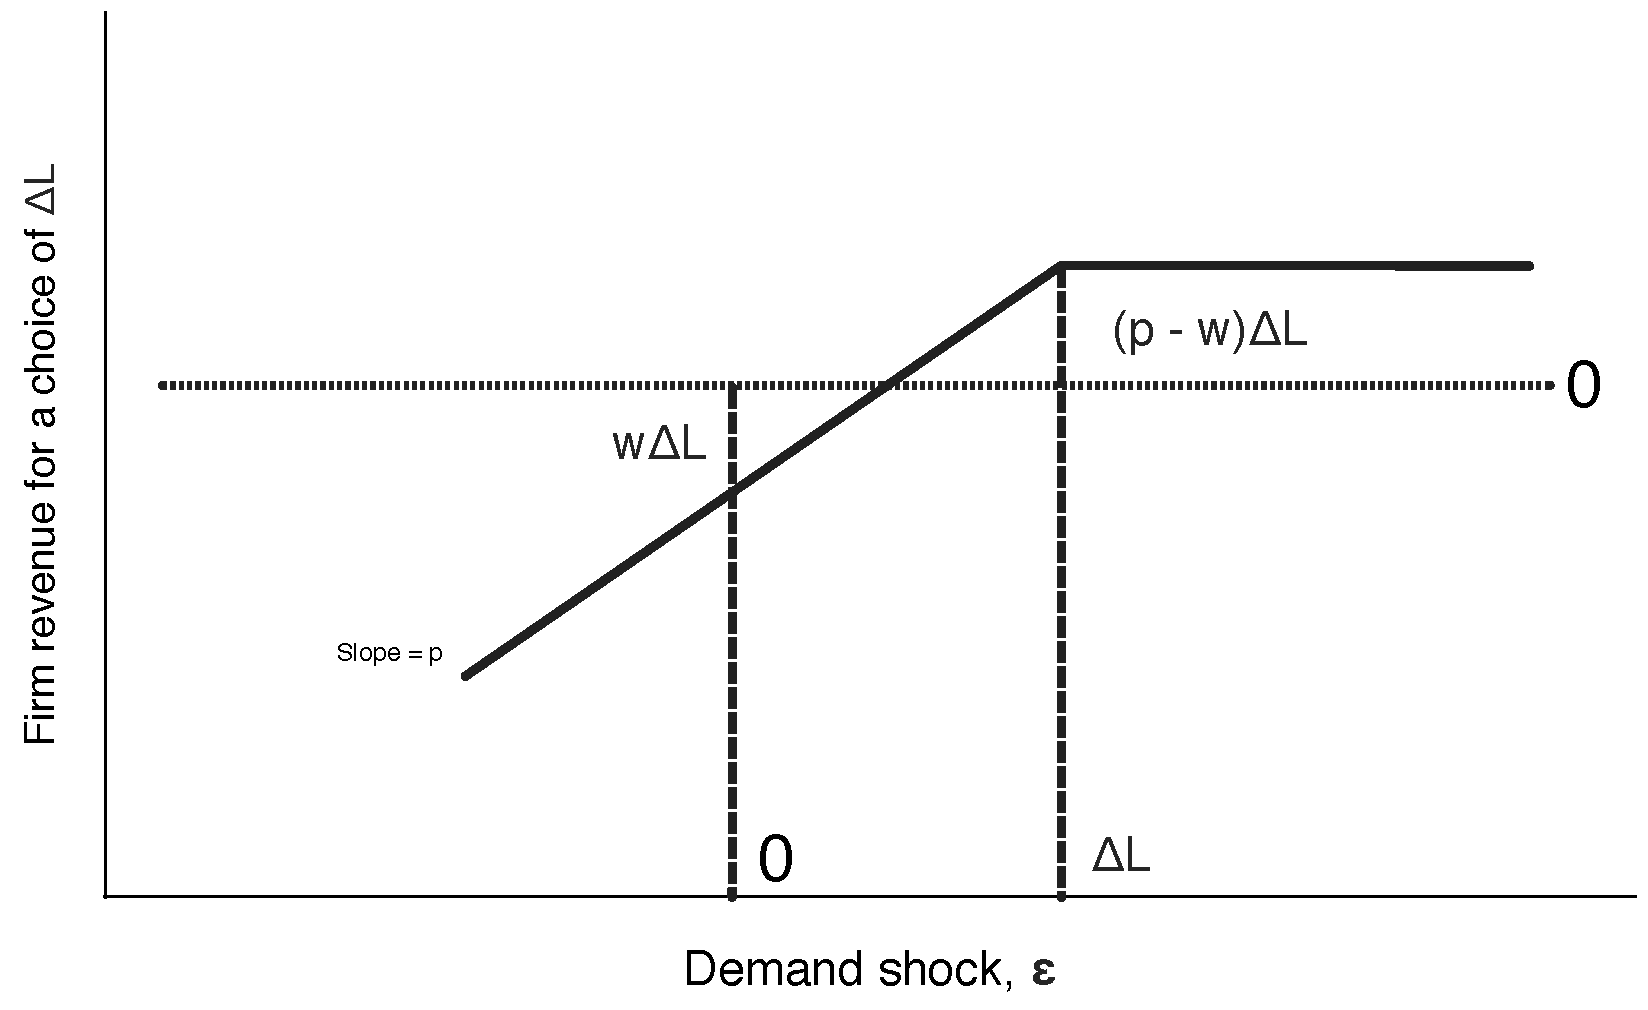
\includegraphics[width = \linewidth]{./diagrams/firms_optimization_problem.pdf}
\\
\emph{Notes}: This figure illustates the firm's change in revenue from different realizations of $\epsilon$, which are demand
shocks. 
\end{minipage} 
\end{figure}

The labor cost is always $\Delta L$.
The firm's change in profit as a function of $\Delta L$ is 
\begin{align}
  \Delta \pi & = \int_{-\infty}^{\Delta L} p \epsilon f(\epsilon) d\epsilon + \int_{\Delta L}^\infty p \Delta L f(\epsilon) d\epsilon - w \Delta L \nonumber \\
             & = \int_{-\infty}^{\Delta L} p \epsilon f(\epsilon) d\epsilon + p \Delta L \left(1 - F(\Delta L) \right) - w \Delta L
\end{align} 
The first order condition is
\begin{align}
  p \Delta L f(\Delta L) + p \left(1 - F(\Delta L)\right) - p \Delta L f(\Delta L) - w & = 0 \nonumber \\
  p \left(1 - F(\Delta L)\right) - w & = 0 \nonumber 
\end{align} 
And so the the firm's optimal labor adjustment is
\begin{align}
 1 - F(\Delta L^*) = \frac{w}{p}.  
\end{align} 

The expression for $\Delta L^*$ has a number of intuitive comparative statics.
When $w$ is relatively high, $\Delta L$ goes down, meaning that the firm uses less labor.
Similarly, when $p$ goes up, the firm uses more labor.
The firm over-staffs if $w < 2p$ and under-staffs when $w > 2p$. 

% http://www.bls.gov/opub/ils/pdf/opbils05.pdf

\subsection{Effects on firm profits from making a staffing adjustment}
In the absence of any adjustment ($\Delta L = 0$), the firm earns profits
\begin{align} 
\int_{-\infty}^{0} p \epsilon f(\epsilon) d\epsilon < 0. 
\end{align} 
This is negative, as the firm  has lost sales for $\epsilon < 0$ but does not benefit from demand is higher, $\epsilon > 0$.
When the firm makes the optimal adjustment, profits are
\begin{align}
  \int_{-\infty}^{\Delta L} p \epsilon f(\epsilon) d\epsilon + p \Delta L \left(1 - F(\Delta L) \right) - w \Delta L \nonumber \\
  \int_{-\infty}^{\Delta L} p \epsilon f(\epsilon) d\epsilon + p \Delta L (w/p) - w \Delta L \nonumber \\
   \int_{-\infty}^{\Delta L} p \epsilon f(\epsilon) d\epsilon 
\end{align} 
and so the change in profits from choosing an optimal $\Delta L$ is
\begin{align}
  \Delta \pi & = \int_{-\infty}^{\Delta L} p \epsilon f(\epsilon) d\epsilon - \int_{-\infty}^{0} p \epsilon f(\epsilon) d\epsilon \nonumber \\
             & = p \left| \int_{0}^{\Delta L} \epsilon f(\epsilon) d\epsilon \right|. 
\end{align}
Interestingly the wage level does not enter directly, but only through the effects on $\Delta L$.
Learning forward a bit, for a fixed level of staffing, $\Delta L$, a reduction in $\sigma$ when the distribution is symmetric will raise revenue.
However, $\Delta L$ will also get closer to zero when the variance goes down (as we will see), but the firm would only do this if it offered a greater profit, and so we can conclude that a reduction in demand variance raises profits---or more predictable equals more profitable.  

\subsection{Changes in demand precision}
When $\sigma$ goes down, meaning that demand estimates are more precise, the firm will choose a $\Delta L$ closer to $0$.
This can be see in readily in Figure~\ref{fig:sigma}, where the blue line is the old $1 - F(\Delta L)$ curve and the gold curve is the same curve but when $\epsilon$ has a lower variance.  
When $w/p$ is above $1/2$, the firm under-staffs and so when $\sigma$ goes down, demand for labor goes up.
In contrast, when $w/p$ is less than the 1/2, the firm firm was over-staffing and so demand for labor goes down following the precision improvement. 

\begin{figure}[h]
\centering 
\caption{Effects of more precise demand estimation} \label{fig:sigma}
\begin{minipage}{0.75 \linewidth}
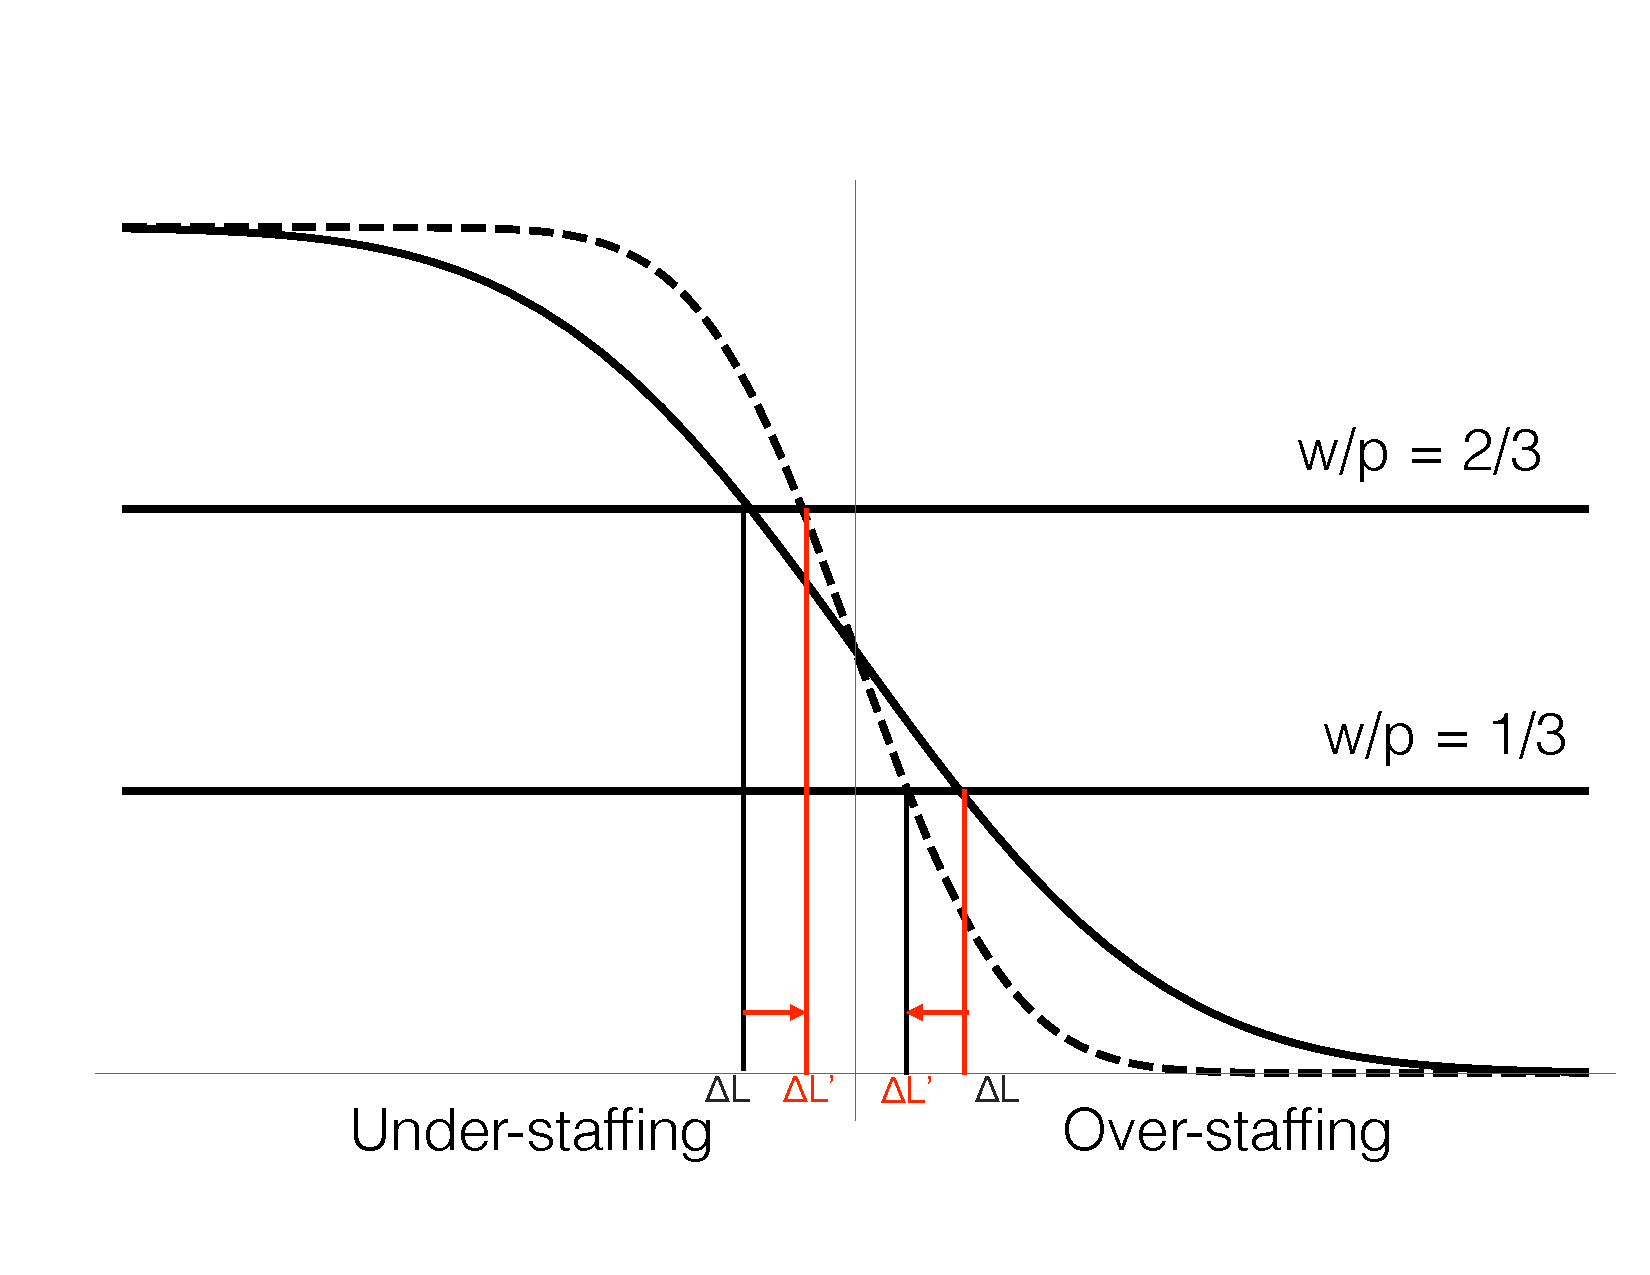
\includegraphics[width = \linewidth]{./diagrams/precision_change.pdf}
\\
\emph{Notes}: This figure illustates the change in labor demand when $\sigma$, the uncertainty in the firm's demand estimation, goes down.  
\end{minipage} 
\end{figure}

\subsection{Transferred variance}
As the firm learns about demand ($\sigma$ goes down), the variance in worker schedules and earnings goes up. 
In a competetive market, the firm would have to pay workers a premium to make them indifferent.

Suppose the firm has a collection of $\bar{L}$ workers.
The probability that a worker works a shift is thus
\begin{align}
\mbox{Pr}(\mbox{work}) = \frac{L + \Delta L}{\bar{L}}. 
\end{align} 

%% \cite{smith1999wealth} had some great ideas! 
%% \important{This is an important claim!}
%% \quantclaim{This is a quantitative claim!} 
%% There a TK important claims in this document. 

\bibliographystyle{aer}
\bibliography{sched.bib}

\end{document} 
